\chapter{Ausarbeitung}
\section{a, b \& c}
\begin{align*}
	A_0 \cos (2\pi\frac{t}{T} + \varphi) = & A_0 \cos(\varphi) \cos(2 \pi \frac{t}{T}) - A_0 \sin (\varphi) \sin(2\pi\frac{t}{T}) \\
	 = & C \cos(2 \pi \frac{t}{T}) + S \sin(2\pi\frac{t}{T})
\end{align*}
wobei $C = A_0 \cos(\varphi)$ und $S = - A_0 \sin (\varphi)$ Konstanten sind. \\\\
Design Matrix $A$:
\begin{equation}
	\bm{A} = \left[t\quad 1 \quad \cos(2 \pi \frac{t}{12}) \quad \sin(2\pi\frac{t}{12})\right]
\end{equation}
Dann sind $a$, $b$, $C$, $S$ mit LS bestimmt werden können. Die Daten Gap ist dann mit gerechnete Parametern ausgefüllt. Das Ergebnis liegt in \autoref{fig:daten}
\begin{figure}[htpb]\centering
	\subfigure[Daten]{
		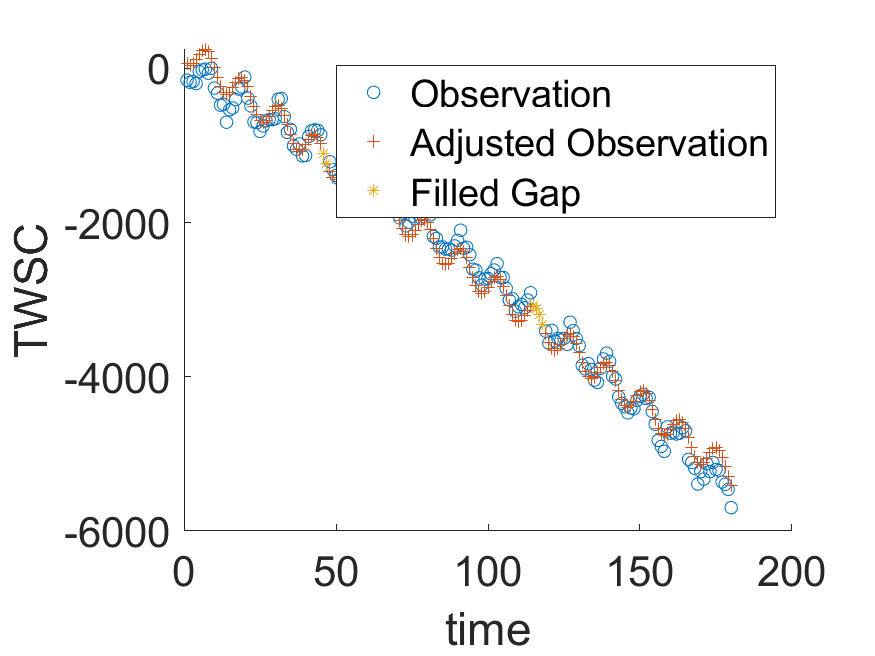
\includegraphics[width=0.9\textwidth]{gapfilling.png}}
	\caption{}
	\label{fig:daten}
\end{figure}
\clearpage
Die 4 Parameter:
\begin{itemize}
	\item $a = -30.77$
	\item $b = 277.9805$
	\item $C = -143.2115$
	\item $S = -126.5081$  
\end{itemize}
Die Var-Kovarianz Matrix von 4 Parameter:
\begin{equation*}
	\Sigma_{xx} = \begin{bmatrix}
		0.0497 & -4.5015 & -0.0973 & 0.1802 \\
		-4.0515 & 544.2370 & 9.6243 & -23.6028 \\
		-0.0973 & 9.6243 & 271.0922 & -1.7560 \\
		0.1802 & -23.6028 & -1.7560 & 276.6499
	\end{bmatrix}
\end{equation*}
\section{d}
\begin{equation*}
	\bm{\hat{x}} = \begin{bmatrix}
		-30.7799 \\
		277.9805 \\
		-143.2115 \\
		-126.5081
	\end{bmatrix}
\end{equation*}
\begin{gather*}
	\bm{\hat{x}_{MAP}} = (\bm{A^{T}} \bm{\Sigma_{yy}^{-1}} \bm{A} + \bm{\Sigma_{xx}^{-1}})^{-1}(\bm{A^{T}}\bm{\Sigma_{yy}^{-1}}\bm{y} + \bm{\Sigma_{xx}^{-1}}\bm{\hat{x}}) \\
	\bm{D} = (\bm{A^{T}} \bm{\Sigma_{yy}^{-1}} \bm{A} + \bm{\Sigma_{xx}^{-1}})^{-1}
\end{gather*}
\begin{equation*}
	\bm{\hat{x}_{MAP}} = \begin{bmatrix}
		-30.8050 \\
		306.7204 \\
		-141.4624 \\
		-125.1237
	\end{bmatrix}
\end{equation*}
\begin{equation*}
	\bm{D} = \begin{bmatrix}
		0.0013 & -0.1140 & -0.0029 & 0.0042 \\
		-0.1140 & 13.2469 & 0.2804 & -0.6382 \\
		-0.0029 & 0.2804 & 5.8076 & -0.0407 \\
		0.0042 & -0.6382 & -0.0407 & 5.9796
	\end{bmatrix}
\end{equation*}
Graph in \autoref{fig:paradist}
\begin{figure}[htpb]\centering
	\subfigure[]{
		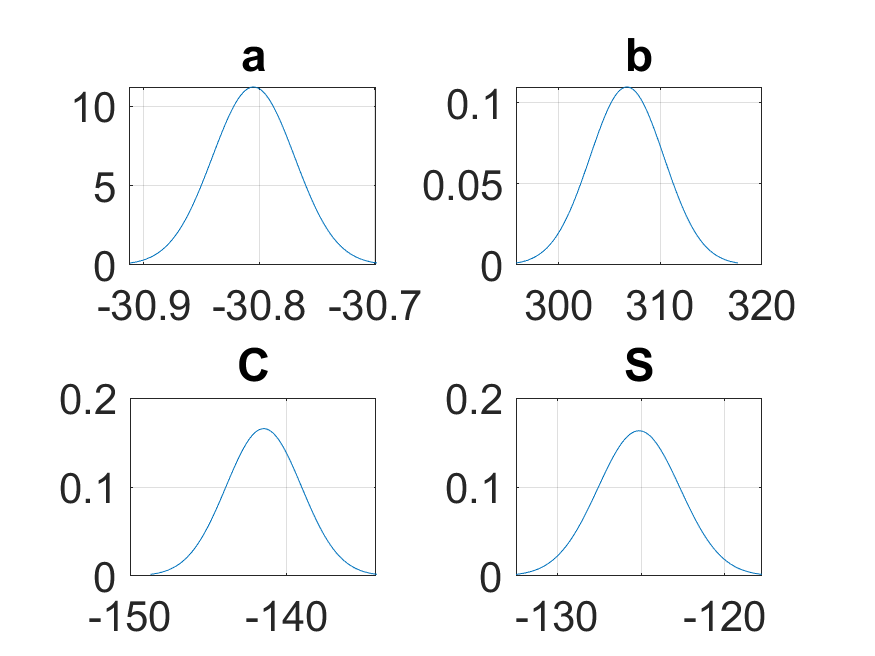
\includegraphics[width=0.9\textwidth]{paradist.png}}
	\caption{}
	\label{fig:paradist}
\end{figure}\\
\section{e}
\begin{equation*}
	\lambda = \frac{\Sigma_x^{-1}}{\Sigma_y^{-1}}
\end{equation*}
Man kann entweder $\Sigma_x^{-1}$ verkleinern oder $\Sigma_y^{-1}$ vergrößern.
\section{f}
$p(y'|T,t,y) = \int p(y'|T,x) p(x|t,y)dx$
\begin{figure}[htpb]\centering
	\subfigure[]{
		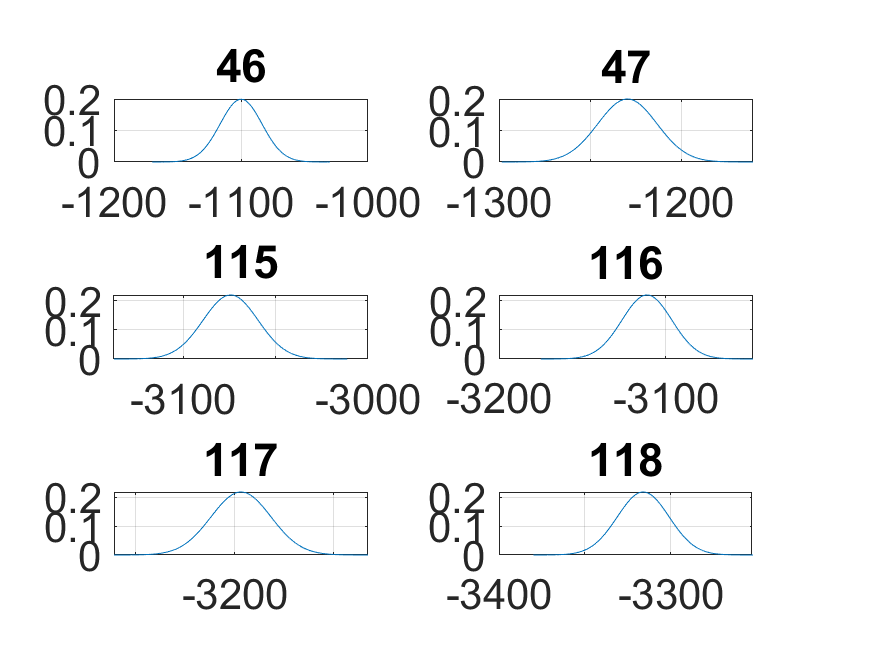
\includegraphics[width=0.9\textwidth]{paradist2.png}}
	\caption{}
	\label{fig:paradist2}
\end{figure}
\clearpage
\section{}
Wiederholt man die obigen Schritten, dieses Mal mit:
\begin{equation*}
	\bm{A} = \left[t^2\quad t \quad  1 \quad \cos(2 \pi \frac{t}{12}) \quad \sin(2\pi\frac{t}{12})\right]
\end{equation*}
Das Verhältnis:
\begin{equation*}
	\frac{prob(M_1 | data)}{prob(M_2 | data)} = \frac{prob(data|M_1)prob(M_1)}{prob(data|M_2)prob(M_2)}
\end{equation*}
Angenommen, dass $prob(M_1) = prob(M_2)$, wenn wir keine Vorwissen haben.
\begin{equation*}
	prob(data|M_1) = \int prob(data|M1,a,b,C,S) \cdot prob(a,b,C,S|M1) dadbdCdS
\end{equation*}
ähnlich für $M?2$, ohne Prior Vorwissen ist diese Aufgabe sehr schwierig zu lösen. 